\documentclass[a4paper, 11pt]{article}
\usepackage{graphicx}
\graphicspath{ {./} }
\usepackage{amsmath, nccmath}

\title{Relazione Progetto Programmazione Avanzata}
\author{Kevin Bernardi Matr. 1058019}
\date{}
\begin{document}
\maketitle
\section{Progetto C++}
\subsection{Introduzione}
Il progetto sulla parte di C++ consiste in una piccola applicazione per tenere traccia di squadre, giocatori, allenatori e delle loro statistiche per il popolare videogioco online competitivo \textit{"Counter Strike: Global Offensive"}, noto anche con l'abbreviazione \textit{"CS:GO"} o \textit{"CSGO"}.

\subsection{Breve panoramica su CSGO}
CSGO è un videogioco online competitivo a squadre di 5 giocatori. Ogni partita si svolge tra due squadre per un massimo di 30 round divisi in 2 tempi da 15 round ciascuno.
La squadra che vince un round guadagna 1 punto e la prima che arriva a 16 round vinti e quindi 16 punti, si aggiudica la vittoria (alla meglio di 30). Se una squadra vince ogni round del primo tempo (15-0) e il primo round del secondo tempo (16-0) la partita termina. Se entrambe le squadre arrivano a 15 punti (punteggio 15 a 15), si procede ad oltranza con i round supplementari.
All'inizio della partita una squadra ha il ruolo di terrorista (\textbf{T}) mentre l'altra quello di anti-terrorista (\textbf{CT}). I ruoli assunti dalle squadre rimangono fissi per l'intero tempo. Prima del round 16, quindi prima dell'inizio del secondo tempo, i ruoli vengono invertiti.
La vittoria di ogni round e la conseguente assegnazione del punto avviene in questo modo:
\begin{itemize}
\item La squadra \textbf{T} può vincere il round facendo esplodere una bomba che deve essere piazzata in una delle 2 zone fisse e specifiche all'interno della mappa o altrimenti eliminando gli avversari entro lo scadere del tempo. La bomba può essere piazzata una sola volta per round;

\item La squadra \textbf{CT} per vincere deve evitare che esploda la bomba piazzata dall'altra squadra oppure eliminare tutti gli avversari prima che piazzino la bomba o disinnescando la bomba una volta piazzata, anche se sono rimasti vivi alcuni giocatori della squadra T.
\end{itemize}



\subsection{Metriche}
Come accennato nell'introduzione, il programma serve a raccogliere le statistiche di giocatori, squadre e allenatori per mostrare delle statistiche aggregate ed effettuare dei confronti per determinare, ad esempio, il miglior giocatore, squadra o allenatore.
I giocatori vengono valutati utilizzando la metrica \textit{\textbf{"Average Kills/Deaths ratio per match"}} abbreviato come \textit{\textbf{"AvgKD"}} calcolato con la seguente formula:
\begin{displaymath}
AvgKD(p) = \frac{ \sum_{m\in matches} \left(\mfrac{kills(m,p)}{deaths(m,p)}\right)}{\#matches}
\end{displaymath}

dove $matches$ è la lista delle partite giocate da un giocatore, $kills(m,p)$ restituisce il numero di eliminazioni della partita $m$ per il giocatore $p$ e $deaths(m,p)$, analogamente, restituisce il numero di morti durante una partita di un giocatore.
Un valore più elevato di questa metrica corrisponde ad un giocatore migliore.
Per quanto riguarda gli allenatori (coach), viene utilizzata una metrica molto simile chiamata \textit{\textbf{"Coach Rating"}} calcolata con la seguente formula:

\begin{displaymath}
Rating(c) = \frac{ \sum_{m\in matches} \left(\mfrac{\sum_{p\in players(m)} \left(\mfrac{kills(m,p)}{deaths(m,p)}\right)}{\#players}\right)}{\#matches}
\end{displaymath}

dove $c$ è un allenatore e $players(m)$ è la lista dei giocatori di una partita (m).
In altri termini il \textit{Coach Rating} è la media (sulle partite) delle medie dei rapporti uccisioni/morti di ogni giocatore nella partita. Anche in questo caso un valore più alto della metrica indica un coach migliore.

\subsection{Struttura del programma}

Il programma è composto dalle seguenti classi:
\begin{itemize}
\item \textbf{Organization}: rappresenta una squadra, contiene i giocatori e l'allenatore che fanno parte della squadra;
\item \textbf{Person}: rappresenta una persona generica con un nome, cognome ed età;
\item \textbf{Coach}: rappresenta un allenatore, può essere assegnato ad una squadra;
\item \textbf{Player}: rappresenta un giocatore professionista, può essere assegnato ad una squadra insieme ad altri giocatori;
\item \textbf{Retired}: rappresenta un giocatore oppure un allenatore che si è ritirato dalle competizioni definitivamente, non può più essere assegnato ad organizzazioni e non può più disputare partite;
\item \textbf{playerMatch}: rappresenta un contenitore con le statistiche di un giocatore in una partita (uccisioni, assist, morti, rapporto k/d).
\end{itemize}
Il funzionamento dettagliato di ogni classe, funzione e metodo è spiegato all'interno del codice mentre l'elenco delle classi, dei loro campi e metodi sono rappresentati nel seguente diagramma UML:

\begin{center}
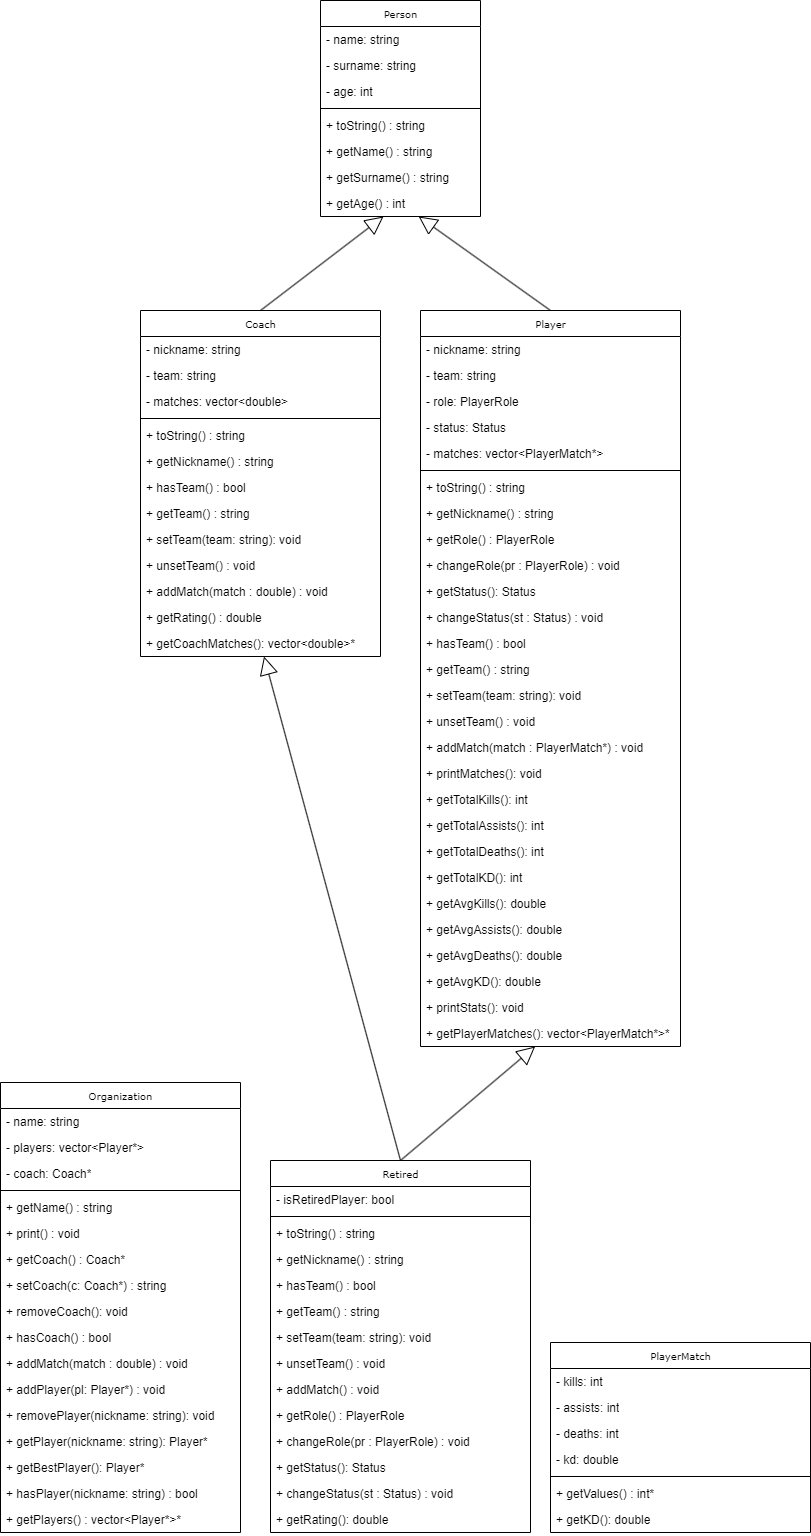
\includegraphics[height=\textheight]{uml}
\end{center}


\section{Progetto Haskell}
\subsection{Introduzione}
Il progetto in Haskell consiste in un programma che conta le occorrenze delle parole in una pagina web passata in input attraverso il terminale appena dopo aver avviato il programma.
Per realizzare il progetto sono state utilizzate le librerie \textit{"Scalpel"} uno web scraper per estrarre testo dalle pagine web e \textit{"split"} per utilizzare metodi aggiuntivi di manipolazione delle liste come \textit{splitOn()} che consente di dividere una stringa in una lista di sottostringhe per separare le parole contenute nelle frasi.

\subsection{Funzionamento del programma}
Per contare le occorrenze delle parole contenute nella pagina web passata in input, il programma esegue i seguenti passi:
\begin{enumerate}
\item ottieni l'URL della pagina su cui far funzionare lo scraper;
\item effettua lo scraping della pagina ed estrai il testo contenuto nei tag \textit{p}, il risultato di questa operazione è una lista di stringhe, una stringa per ogni tag \textit{p};
\item fondi le diverse stringhe in un'unica stringa;
\item spezza l'unica stringa per creare una lista di parole;
\item conta le occorrenze e ordinale andando a creare una lista di tuple di arietà 2:

\textit{esempio: [(3, "studente"), (2, "informatica"), (2, "ingegneria")];}
\item stampa il risultato.

\end{enumerate}

\end{document}

